\subsection{Pisa/IIT SoftHand}
\label{sec:softhand}

The Pisa/IIT SoftHand is a 5-finger hand that introduces an implementation of the adaptive synergy transmission~\cite{Catalano2014Adaptive}. Fig~\ref{fig:soft_hand}.

\begin{figure}
\centering
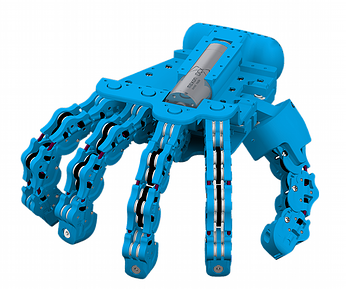
\includegraphics[width=0.4\textwidth]{soft_hand.png}
\caption{The Pisa/IIT SoftHand, 1 motor and 19 dof.}
\label{fig:soft_hand}
\end{figure}

\subsubsection{Hardware interface}

The real hardware interface is implemented wrapping the API provided by qbrobotics$^{\copyright}$~\cite{qbrobotics_software}.

\paragraph{Transmission interface}

\subsubsection{Joint state estimation}

At this point, there are two on going works regarding this issue that we expect to converge to sensor fusion approach during the time remaining on the project. The first one is presented in DR 3.1, where an IMU-based glove provides an accurate estimate of the joint angles. The second approach is a simulator-in-the-loop extended kalman filter, where the simulation takes the place of the system model to give the estimated joint values, and motor position (via a position encoder) and effort (estimated from the current measurement) are used as measurements to update the filter via the adaptive synergy transmission equations implemented in the transmission interface as described above. This work is being submitted to IROS 2015, for more details see the attached at~\href{}{this link}.